% This is the code that generates the slides we'll use for this section.
% If you'd simply like to view the slides, please open slides.pdf


\documentclass[10pt, aspectratio=169]{beamer}

\makeatletter
  \def\beamer@calltheme#1#2#3{%
    \def\beamer@themelist{#2}
    \@for\beamer@themename:=\beamer@themelist\do
    {\usepackage[{#1}]{\beamer@themelocation/#3\beamer@themename}}}

  \def\usefolder#1{
    \def\beamer@themelocation{#1}
  }
  \def\beamer@themelocation{}

\usefolder{../__resources__/beamer_theme}
\usetheme{nathan}

\addtobeamertemplate{navigation symbols}{}{%
    \usebeamerfont{footline}%
    \usebeamercolor[fg]{footline}%
    \hfill%
    \insertframenumber/\inserttotalframenumber
}

\title{Computational Decision Making for Regular People}
\subtitle{01: Introduction}
\date{October 15, 2024}

\usepackage[font=tiny,labelfont=bf]{caption}
\usepackage{caption}
\captionsetup[figure]{labelformat=empty}

\begin{document}

\begin{frame}
    \maketitle
\end{frame}

\begin{frame}{Today's Outline}
    \begin{columns}
        \begin{column}{0.5\textwidth}
            \begin{enumerate}
                \item Mathematical Modeling
                \item Optimization
                \item What kinds of things can be optimized?
                \item General form of an optimization problem
                \item A note on optimization theory
                \item How to formulate an optimization problem
                \begin{enumerate}
                    \item The objective function
                    \item Decision variables
                    \item Parameters
                    \item Constraints
                \end{enumerate}
                \item Basic Examples
            \end{enumerate}
        \end{column}
        \begin{column}{0.5\textwidth}
            \begin{figure}
                
\includegraphics[width=0.95\linewidth]{Brain.jpeg}
                \caption{This image was created with the assistance of DALL·E 3}
            \end{figure}
        \end{column}
    \end{columns}
\end{frame}

\begin{frame}{Mathematical Modeling}
    \begin{tabular}[t]{p{6.5cm} | p{6.5cm}}
        How we think about a problem & How a computer thinks about a problem \\
        \hline
        \begin{itemize}
            \item Consider what a good outcome looks like
            \begin{itemize}
                \item Consider different ramifications of different decisions 
                \item utilitarian ethics, virtue ethics, deontological ethics, ...
            \end{itemize}
        \end{itemize} & \begin{itemize}
            \item Quantify the quality of a solution
            \begin{itemize}
                \item Combine all ramifications into one quantity
                \item utilitarian objective only*
            \end{itemize}
        \end{itemize} \\
        \begin{itemize}
            \item Discrete decisions (yes/no, 1,2,3, etc.)  
            \item Continuous decisions
            \item Constraints against undesirable or infeasible decisions
        \end{itemize} & \begin{itemize}
            \item Discrete decisions (yes/no, 1,2,3, etc.)  
            \item Continuous decisions
            \item Constraints against undesirable or infeasible decisions
        \end{itemize} \\
    \end{tabular}
\end{frame}

\begin{frame}[t]{Optimization}
    \textit{the action of making the best or most effective use of a situation or resource.}\footnote{Oxford Languages}
    \vspace{0.5cm}
    \begin{columns}[t]
        \begin{column}[t]{0.5\textwidth}
            \begin{itemize}
                \item Given a set of possible decisions, determine the best one(s)
                \item The way this determination is made depends on the nature of the set of decisions
                \begin{itemize}
                    \item If a human is executing this determination, the procedure will be unique to that person
                    \item If a computer algorithm is executing this determination, the procedure will be unique to that computer algorithm
                \end{itemize}
            \end{itemize}
        \end{column}
        \begin{column}[t]{0.5\textwidth}
            \begin{figure}
                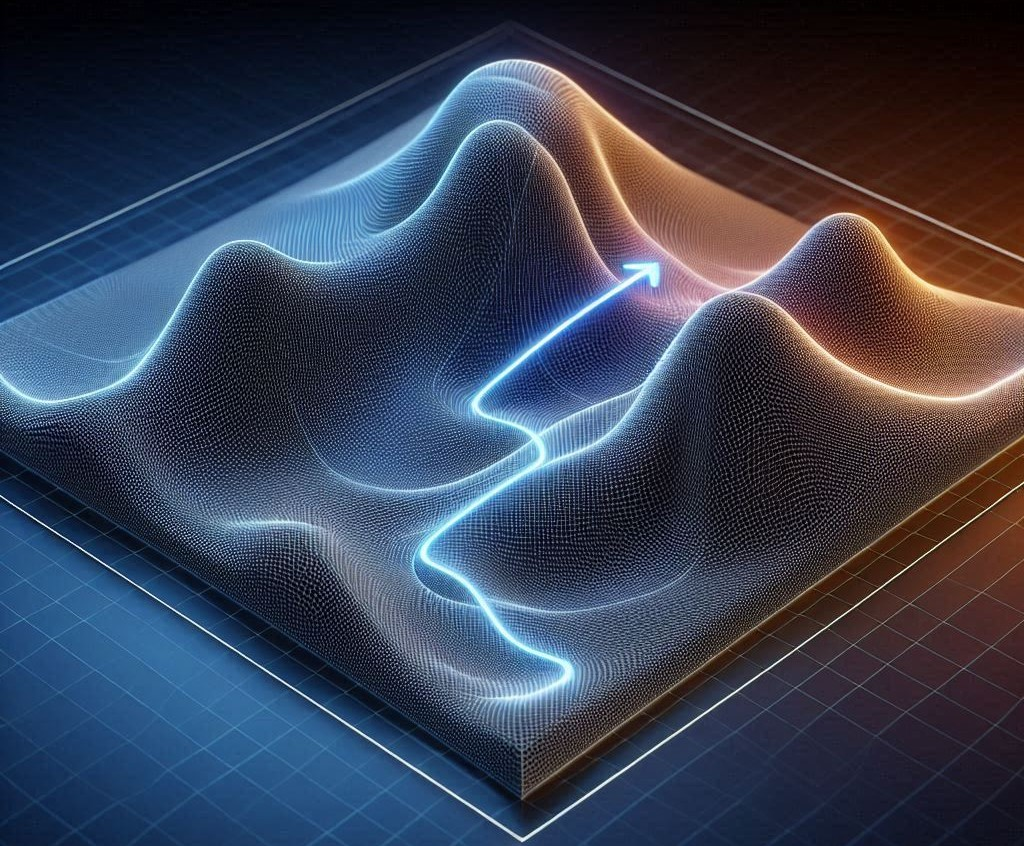
\includegraphics[width=0.8\linewidth]{Mountain.jpeg}
                \caption{This image was created with the assistance of DALL·E 3}
            \end{figure}
        \end{column}
    \end{columns}
\end{frame}

\begin{frame}{What Kinds of Things Can Be Optimized?}
    \begin{itemize}
        \item What kinds of things can be optimized (using a computer)?
        \item If you can represent it using mathematical modeling, it (theoretically) can be optimized.
        \item Some problems are still too difficult for even modern computer algorithms to solve
        \begin{itemize}
            \item Problems with lots and lots of variables
            \item Problems with lots and lots of constraints
            \item Problems that "don't behave well"
            \begin{itemize}
                \item Lots of really good outcomes that lie very close to really bad outcomes
                \item Lots of outcomes that are equally good
                \item Good outcomes that are separated by bad outcomes
                \item Really nuanced constraints
                \item etc.
            \end{itemize}
        \end{itemize}
    \end{itemize}
\end{frame}

\begin{frame}{General Form of an Optimization Problem}
    \begin{columns}
        \begin{column}{0.5\textwidth}
            $$\min f(\overline{X})$$
            $$---\ subject\ to\ (s.t.)\ ---$$
            $$\overline{X} \in \textbf{S}$$
            \vspace{1cm}
            \begin{itemize}
                \item We must define:
                \begin{itemize}
                    \item $\overline{X}$
                    \item $f(\overline{X})$
                    \item $\textbf{S}$
                \end{itemize}
            \end{itemize}
        \end{column}
        \begin{column}{0.5\textwidth}
            \begin{figure}
                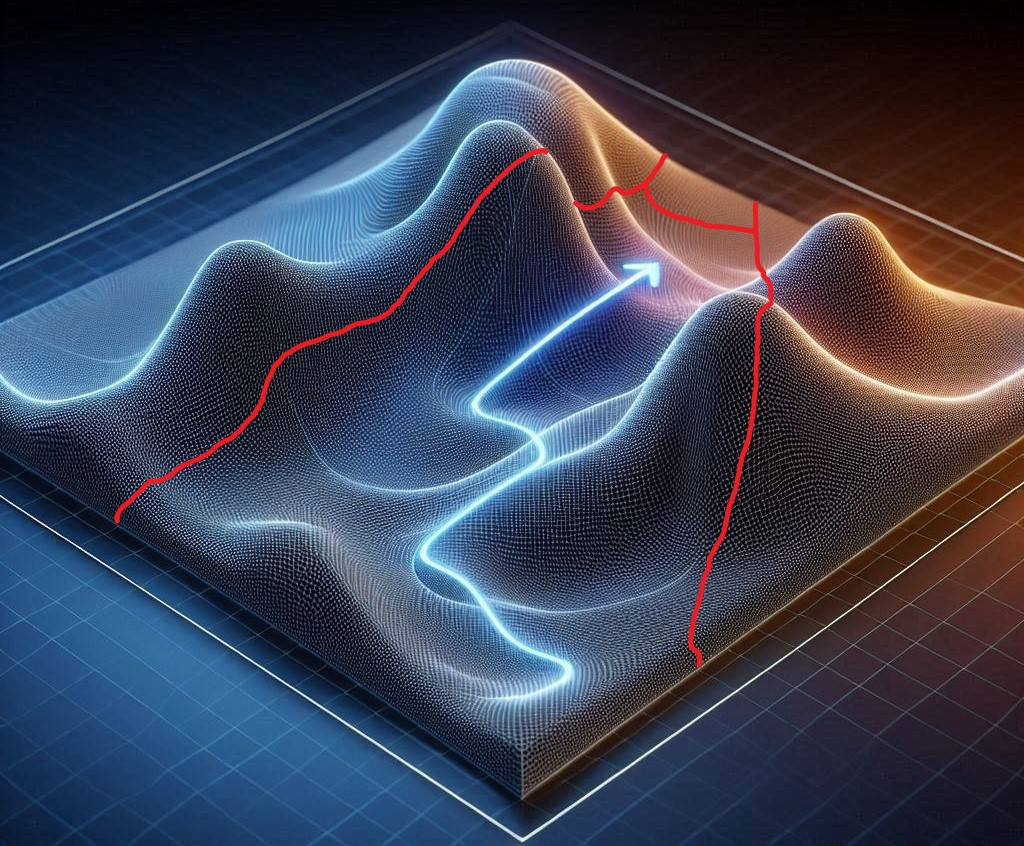
\includegraphics[width=\linewidth]{MountainWithFences.jpg}
            \end{figure}
        \end{column}
    \end{columns}
\end{frame}

\begin{frame}[t]{Optimization Theory}
    \begin{columns}[t]
        \begin{column}[t]{0.5\textwidth}
            \begin{itemize}
                \item This is a very active field of research
                \item It gets quite complicated and "mathy" very quickly
                \item  I'll only emphasize two points:
            \end{itemize}
            \vspace{0.5cm}
            \begin{center}
                \textbf{If we can keep $f(\overline{X})$ and $\textbf{S}$ as linear as possible, the computer algorithms are MUCH faster.}
                
                \vspace{0.4cm}
                
                \textbf{If we can't keep things linear, "Bilinear" is the next best thing.}
            \end{center}
        \end{column}
        \begin{column}[t]{0.5\textwidth}
            $$\min f(\overline{X})$$
            $$s.t.\ \overline{X} \in \textbf{S}$$
            \vspace{1cm}
            \begin{itemize}
                \item Linear: $\alpha X + \beta Y + \gamma Z$
                \item Bilinear: $\alpha X Y$ or $\alpha X^2$
                \item Non-linear: 
                \begin{itemize}
                    \item $\alpha\sqrt{X}$
                    \item $\alpha \log{\left(X\right)}$
                    \item etc.
                \end{itemize}
            \end{itemize}
        \end{column}
    \end{columns}
\end{frame}

\begin{frame}{Formulating Optimization Problems}
    Key Elements:
    \vspace{0.5cm}
    \begin{columns}[t]
        \begin{column}[t]{0.5\textwidth}
            In order how I would conceptualize them:
            \begin{enumerate}
                \item Objective Function ($f(\overline{X}$))
                \item Decision Variables ($\overline{X}$)
                \item Parameters ($\overline{\alpha}$)
                \item Constraints ($\textbf{S}$)
            \end{enumerate}
        \end{column}
        \begin{column}[t]{0.5\textwidth}
            In order how I would write / code them:
            \begin{enumerate}
                \item Parameters ($\overline{\alpha}$)
                \item Decision Variables ($\overline{X}$)
                \item Constraints ($\textbf{S}$)
                \item Objective Function ($f(\overline{X}$))
            \end{enumerate}
        \end{column}
    \end{columns}
\end{frame}

\begin{frame}{Objective Function ($f(\overline{X}$))}
    \begin{columns}
        \begin{column}{0.5\textwidth}
            \begin{itemize}
                \item What am I trying to accomplish?
                \item What am I trying to minimize (or maximize)?
                \item How do different decisions change the outcome?
            \end{itemize}
            Examples:
            \begin{itemize}
                \item Minimize cost
                \item Minimize risk
                \item Maximize probability of reaching a goal
                \item Maximize comfort
            \end{itemize}
        \end{column}
        \begin{column}{0.5\textwidth}
            \begin{figure}
                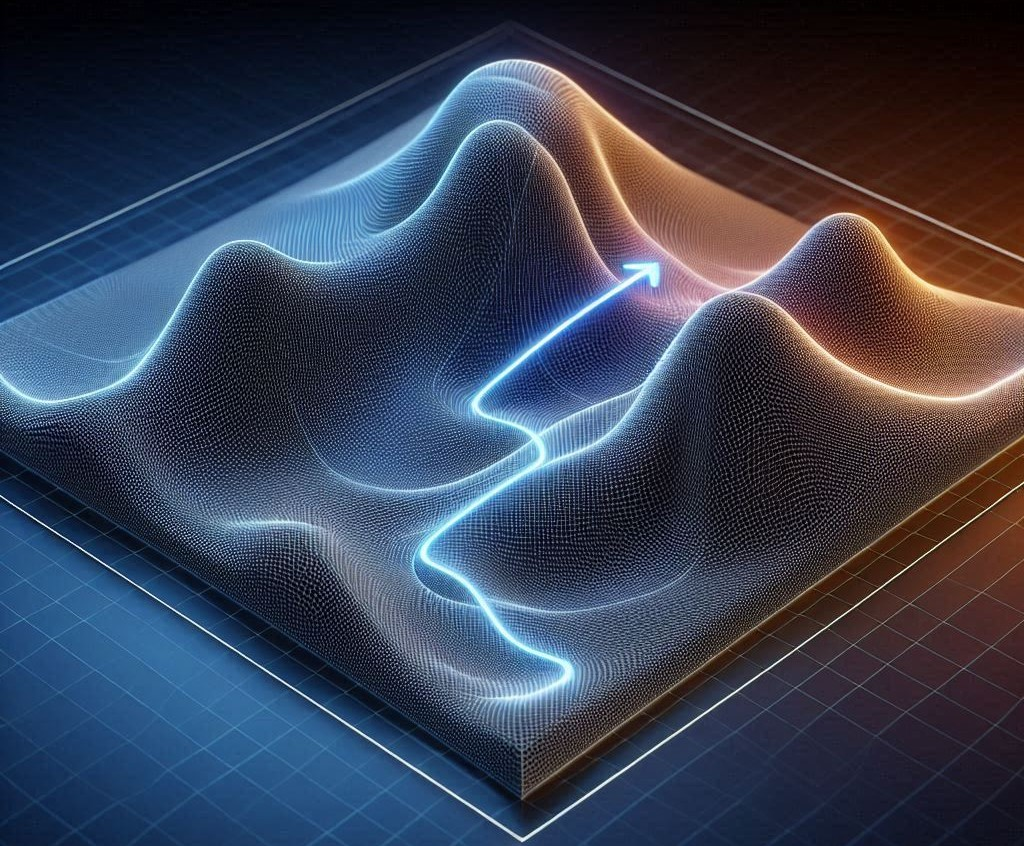
\includegraphics[width=0.8\linewidth]{Mountain.jpeg}
            \end{figure}
        \end{column}
    \end{columns}
\end{frame}

\begin{frame}{Decision Variables ($\overline{X}$)}
    \begin{columns}
        \begin{column}{0.5\textwidth}
            \begin{itemize}
                \item What decisions can I make?
                \item What values change when I make different decisions?
            \end{itemize}
            Important Note:
            \begin{itemize}
                \item Be open-minded here: often the best way to formulate a problem is to consider each individual part of a problem as it's own variable.
                \item Don't just consider the main decisions, consider the smaller decisions that contribute to (or even strictly define) the main decisions
            \end{itemize}
            Examples:
            \begin{itemize}
                \item How much of a certain item to buy
                \item How much of a budget category to allot for that item
                \item 
            \end{itemize}
        \end{column}
        \begin{column}{0.5\textwidth}
            \begin{figure}
                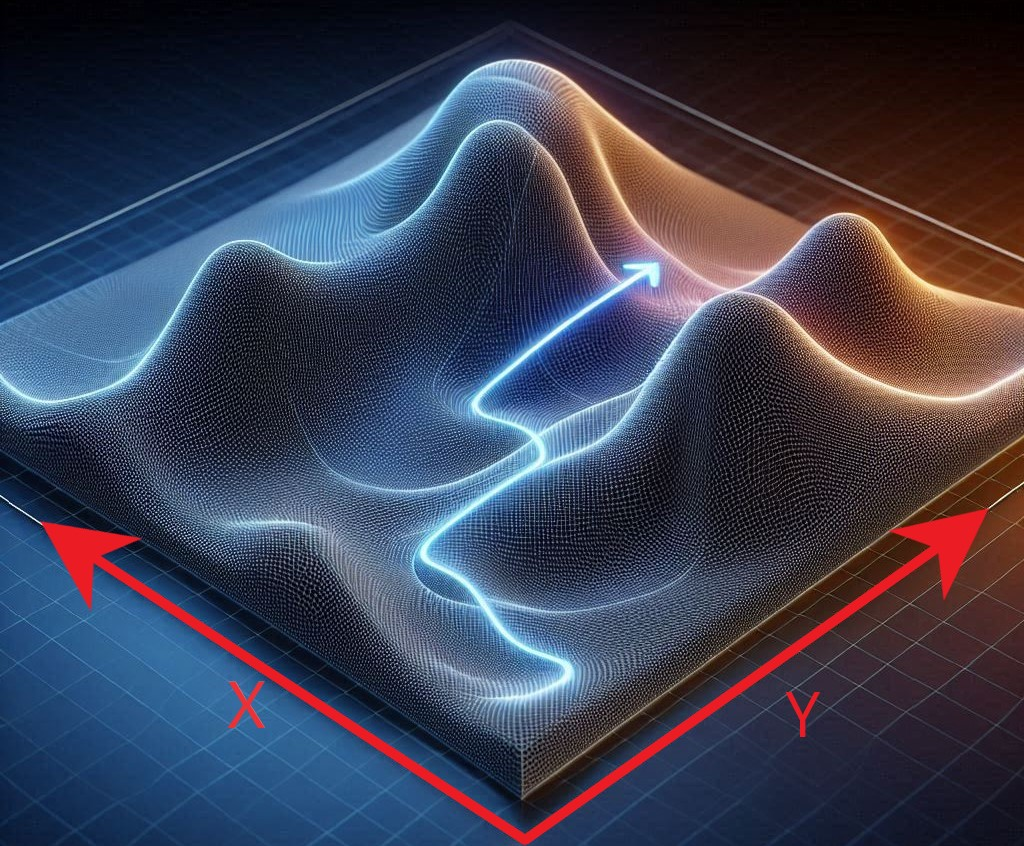
\includegraphics[width=0.8\linewidth]{MountainWithDecisionVariables.jpeg}
            \end{figure}
        \end{column}
    \end{columns}
\end{frame}

\begin{frame}{Parameters ($\overline{\alpha}$)}
    \begin{columns}
        \begin{column}{0.5\textwidth}
            \begin{itemize}
                \item What parts of the problem are fixed or immovable?
                \item While the Objective function defines the general shape of the mountain, the parameters define the height of the peaks, the steepness of the slopes, etc.
            \end{itemize}
            Examples:
            \begin{itemize}
                \item Cost of a certain item
                \item Total amount of time available
                \item The minimum probability of reaching a goal that we are willing to accept
            \end{itemize}
        \end{column}
        \begin{column}{0.5\textwidth}
            \begin{figure}
                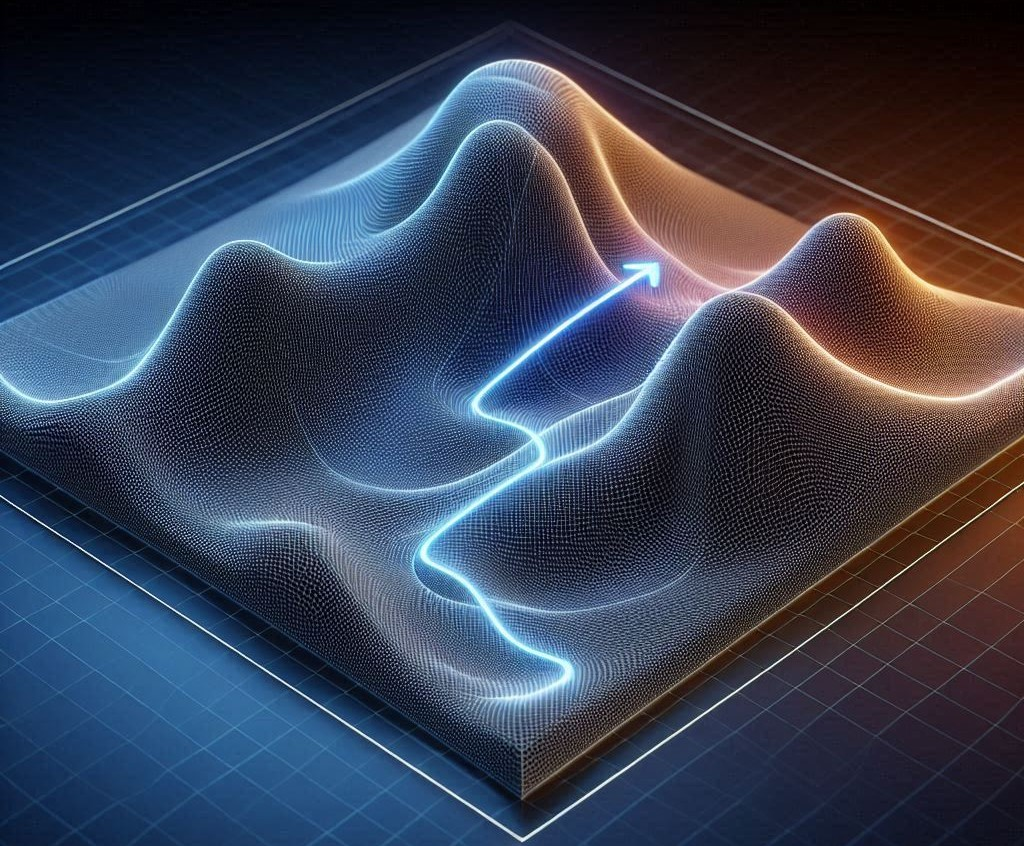
\includegraphics[width=0.8\linewidth]{Mountain.jpeg}
            \end{figure}
        \end{column}
    \end{columns}
\end{frame}

\begin{frame}{Constraints ($\textbf{S}$)}
    \begin{columns}
        \begin{column}{0.5\textwidth}
            \begin{itemize}
                \item What sets of decisions are incompatible?
                \item What is the nature of an individual decision? (Binary, Continuous, etc.)
                \item How do different decision variables relate to each other?
            \end{itemize}
            Examples:
            \begin{itemize}
                \item We cannot spend more in a budget category than the total allotment for that category.
                \item The amount of money spent in a budget category is strictly equal to the sum of transactions that lies in that category.
                \item The calculated probability of reaching a goal must be greater than the minimum value we specified.
            \end{itemize}
        \end{column}
        \begin{column}{0.5\textwidth}
            \begin{figure}
                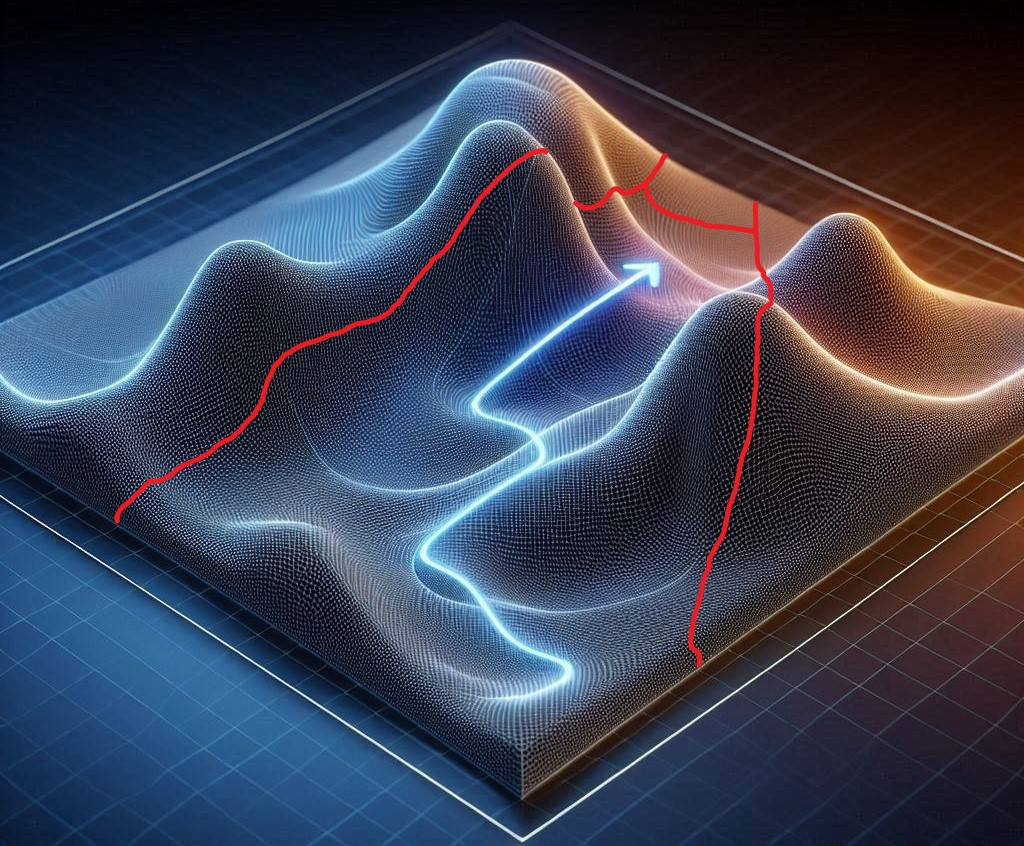
\includegraphics[width=0.8\linewidth]{MountainWithFences.jpg}
            \end{figure}
        \end{column}
    \end{columns}
\end{frame}

\begin{frame}{A Visual Example (Linear)}
    %Do a 2-d visual example (maybe one linear and one non-linear)
    \begin{columns}
        \begin{column}{0.5\textwidth}
            \begin{figure}
                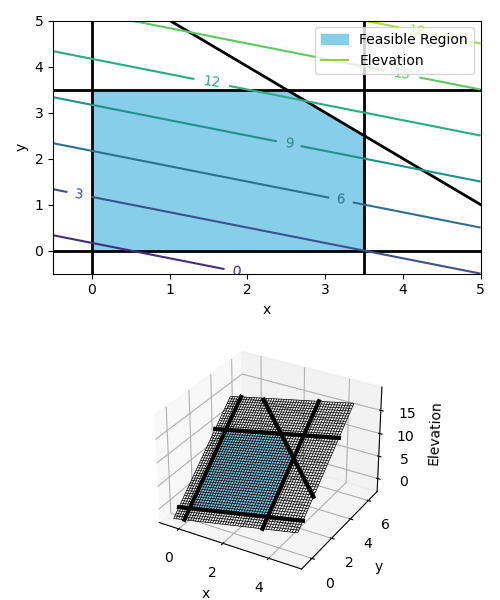
\includegraphics[width=0.8\linewidth]{LinearObjective.png}
            \end{figure}
        \end{column}
        \begin{column}{0.5\textwidth}
            $$\max X + 3Y - 0.5$$
            $$s.t. \ \ \ X\geq 0$$
            $$Y \geq 0$$
            $$X \leq 3.5$$
            $$Y \leq 3.5$$
            $$X + Y \leq 6$$
        \end{column}
    \end{columns}
\end{frame}

\begin{frame}{A Visual Example (Nonlinear)}
    %Do a 2-d visual example (maybe one linear and one non-linear)
    \begin{columns}
        \begin{column}{0.5\textwidth}
            \begin{figure}
                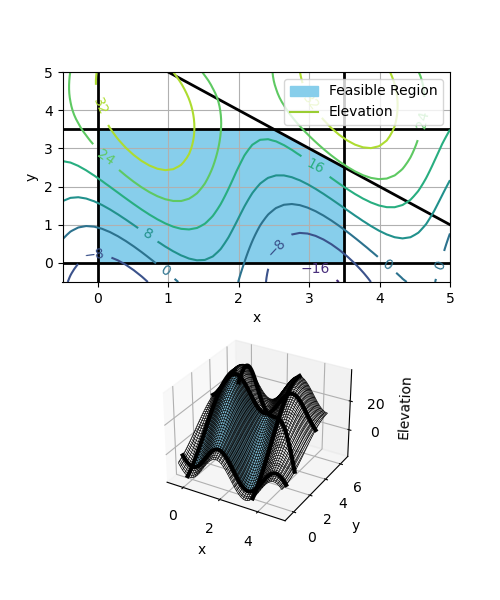
\includegraphics[width=0.9\linewidth]{NonlinearObjective.png}
            \end{figure}
        \end{column}
        \begin{column}{0.5\textwidth}
            $$\max f(X,Y)$$
            $$s.t. \ \ \ X\geq 0$$
            $$Y \geq 0$$
            $$X \leq 3.5$$
            $$Y \leq 3.5$$
            $$X + Y \leq 6$$
        \end{column}
    \end{columns}
\end{frame}

\begin{frame}[t]{Example: Etsy Shop Problem}
    \textit{Jack and Jill own an Etsy shop that sells t-shirts and wooden sculptures. Jack can either make 5 t-shirts per hour or he can make 2 sculptures per hour. Jill can either make 9 t-shirts per hour or she can make 3 sculptures per hour. Their most recent order indicates that they only need 25 t-shirts but would welcome as many sculptures as they can create. They each how 8 hours to work today. How should they spend their time today so that they can maximize the total number of t-shirts and sculptures they make?}

    \vspace{1.0cm}
    
    Take a minute to think about the problem on your own:
    \begin{enumerate}
        \item Objective Function ($f(\overline{X}$))
        \item Decision Variables ($\overline{X}$)
        \item Parameters ($\overline{\alpha}$)
        \item Constraints ($\textbf{S}$)
    \end{enumerate}
\end{frame}

\begin{frame}{Example: Etsy Shop Problem}
    \textbf{First conceptualize the problem:}
    \begin{columns}[t]
        \begin{column}[t]{0.5\textwidth}
            \begin{itemize}
                \item Objective: Maximize the total number of products produced
                \item Variables: 
                \begin{itemize}
                    \item How many hours each person spends on producing each product
                    \item The amount of each product that gets made
                \end{itemize}
                
                \item Parameters: 
                \begin{itemize}
                    \item How much product can be made by each person per hour
                    \item How must time there is in a day
                    \item The number of t-shirts they need
                    \item The priority between each product
                \end{itemize}
            \end{itemize}
        \end{column}
        \begin{column}[t]{0.5\textwidth}
            \begin{itemize}
                \item Constraints:
                \begin{itemize}
                    \item Each person can only work between 0 and 8 hours in a day
                    \item The amount of each product produced should be directly determined by how many hours each person spends making that product
                    \item The number of t-shirts should be limited to 25
                \end{itemize}
            \end{itemize}
        \end{column}
    \end{columns}
\end{frame}

\begin{frame}[t]{Example: Etsy Shop Problem}
    \textbf{Let's write the problem using mathematical modeling:}
    \begin{columns}[t]
        \begin{column}[t]{0.5\textwidth}
            \begin{enumerate}
                \item Define Parameters:
                \begin{itemize}
                    \item How much product can be made by each person per hour
                    \begin{itemize}
                        \item $\alpha_{Jack,Sculptures} = 2$
                        \item $\alpha_{Jack,Shirts} = 5$
                        \item $\alpha_{Jill,Sculptures} = 3$
                        \item $\alpha_{Jill,Shirts} = 9$
                    \end{itemize}
                    \item $\tau^{DAY} = 8$: How much time there is to work in a day
                    \item $\kappa = 25$: The number of t-shirts they need
                \end{itemize}
            \end{enumerate}
        \end{column}
        \begin{column}[t]{0.5\textwidth}
            \begin{enumerate}
                \setcounter{enumi}{1}
                \item Define Decision Variables:
                \begin{itemize}
                    \item The number of hours each person should spend making each product in a day
                    \begin{itemize}
                        \item $H_{Jack,Sculptures}$
                        \item $H_{Jack,Shirts}$
                        \item $H_{Jill,Sculptures}$
                        \item $H_{Jill,Shirts}$
                    \end{itemize}
                    \item The amount of each product that gets made
                    \begin{itemize}
                        \item $N_{Sculptures}$
                        \item $N_{Shirts}$
                    \end{itemize}
                \end{itemize}
            \end{enumerate}
        \end{column}
    \end{columns}
\end{frame}

\begin{frame}{Example: Etsy Shop Problem}
    \begin{enumerate}
        \setcounter{enumi}{2}
        \item Constraints:
        \begin{itemize}
            \item Each person can only work between 0 and 8 hours in a day:
            $$0 \leq H_{Jack,Sculptures} + H_{Jack,Shirts} \leq \tau^{DAY}$$
            $$0 \leq H_{Jill,Sculptures} + H_{Jill,Shirts} \leq \tau^{DAY}$$
            \item The amount of each product produced should be directly determined by how many hours each person spends making that product:
            $$N_{Sculptures} = \alpha_{Jack,Sculptures} H_{Jack,Sculptures} + \alpha_{Jill,Sculptures} H_{Jack,Sculptures}$$
            \begin{equation}
                \begin{split}
                    N_{Shirts} = \alpha_{Jack,Shirts} H_{Jack,Shirts} + \alpha_{Jill,Shirts} H_{Jack,Shirts}
                \end{split}
                \tag*{}
            \end{equation}
            \item The number of shirts should be limited to 25:
            $$N_{Shirts} = \kappa$$
        \end{itemize}
        \setcounter{enumi}{3}
        \item Define Objective:
        \begin{itemize}
            \item Maximize the total number of products produced
            $$\max N_{Shirts} + N_{Sculptures}$$
        \end{itemize}
    \end{enumerate}
\end{frame}

\begin{frame}{Example: Etsy Shop Problem}
    \begin{columns}
        \begin{column}{0.6\textwidth}
            \begin{center}
                \textbf{FULL FORMULATION}
        
                $$\max N_{Shirts} + N_{Sculptures}$$
                $$---\ subject\ to\ (s.t.)\ ---$$
                $$0 \leq H_{Jack,Sculptures} + H_{Jack,Shirts} \leq \tau^{DAY}$$
                $$0 \leq H_{Jill,Sculptures} + H_{Jill,Shirts} \leq \tau^{DAY}$$
                $$N_{Shirts} = \alpha_{Jack,Shirts} H_{Jack,Shirts} + \alpha_{Jill,Shirts} H_{Jack,Shirts}$$
                \begin{equation}
                    \begin{split}
                        N_{Sculptures} = \alpha_{Jack,Sculptures} H_{Jack,Sculptures} \\ + \alpha_{Jill,Sculptures} H_{Jack,Sculptures}
                    \end{split}
                    \tag*{}
                \end{equation}
                $$N_{Shirts} = \kappa$$
            \end{center}
        \end{column}
        \begin{column}{0.4\textwidth}
            \begin{itemize}
                \item Notice how much repetition there is.
                \item How could I change this problem if I had 1000 people and 75 products?
            \end{itemize}
        \end{column}
    \end{columns}
\end{frame}


\begin{frame}{Sets}
    \begin{columns}
        \begin{column}{0.5\textwidth}
            \begin{itemize}
                \item Often there are several variables, parameters, constraints, etc. that are repeated for a given set of values.
                \item We can write the general idea behind that variable, parameter, constraint, etc. by simply writing it once and indicating that it should be repeated for every element in a set.
                \item In math, it looks like this:
            \end{itemize}
            $$\forall e \in \textbf{E}$$
            $$"\text{for all elements } e \text{ in the set } \textbf{E}"$$
        \end{column}
        \begin{column}{0.5\textwidth}
            $$0 \leq H_{Jack,Sculptures} + H_{Jack,Shirts} \leq \tau^{DAY}$$
            $$0 \leq H_{Jill,Sculptures} + H_{Jill,Shirts} \leq \tau^{DAY}$$
            $$\downarrow$$
            $$0 \leq H_{p,Sculptures} + H_{p,Shirts} \leq \tau^{DAY} \ \ \forall p \in \textbf{P}$$
            $$\downarrow$$
            $$0 \leq \sum_{r \in \textbf{R}} H_{p,r} \leq \tau^{DAY} \ \ \forall p \in \textbf{P}$$
            \vspace{0.5cm}
            $$p\in\textbf{P}:\text{ A set of all People}$$
            $$r\in\textbf{R}:\text{ A set of all Products}$$
        \end{column}
    \end{columns}
\end{frame}

\begin{frame}{Sets}
    \begin{columns}
        \begin{column}{0.5\textwidth}
            $$\alpha_{Jack,Sculptures} = 2$$
            $$\alpha_{Jack,Shirts} = 5$$
            $$\alpha_{Jill,Sculptures} = 3$$
            $$\alpha_{Jill,Shirts} = 9$$
            $$\downarrow$$
            $$\alpha_{p,r} \ \ \forall p \in \textbf{P}, r \in \textbf{R}$$
            \begin{center}
                \begin{tabular}{|c||c|c|}
                    \hline
                    $\alpha_{p,r}$ & $Jack$ & $Jill$ \\ 
                    \hline \hline
                    $Shirts$ & 5 & 9 \\  
                    \hline
                    $Sculptures$ & 2 & 3\\
                    \hline  
                \end{tabular}
            \end{center}
        \end{column}
        \begin{column}{0.5\textwidth}
            $$N_{Shirts} = \alpha_{Jack,Shirts} H_{Jack,Shirts} + \alpha_{Jill,Shirts} H_{Jack,Shirts}$$
            \begin{equation}
                \begin{split}
                    N_{Sculptures} = \alpha_{Jack,Sculptures} H_{Jack,Sculptures} \\ + \alpha_{Jill,Sculptures} H_{Jack,Sculptures}
                \end{split}
                \tag*{}
            \end{equation}
            $$\downarrow$$
            $$N_{r} = \alpha_{Jack,r} H_{Jack,r} + \alpha_{Jill,r} H_{Jack,r}\ \ \ \forall r \in \textbf{R}$$
            $$\downarrow$$
            $$N_{r} = \sum_{p \in \textbf{P}} \alpha_{p,r} H_{p,r}\ \ \ \forall r \in \textbf{R}$$
        \end{column}
    \end{columns}
\end{frame}

\begin{frame}[t]{Example: Etsy Shop Problem with Sets}
    \begin{columns}[t]
        \begin{column}[t]{0.5\textwidth}
            $$\max N_{Shirts} + N_{Sculptures}$$
            $$---\ subject\ to\ (s.t.)\ ---$$
            $$0 \leq H_{Jack,Sculptures} + H_{Jack,Shirts} \leq \tau^{DAY}$$
            $$0 \leq H_{Jill,Sculptures} + H_{Jill,Shirts} \leq \tau^{DAY}$$
            $$N_{Shirts} = \alpha_{Jack,Shirts} H_{Jack,Shirts} + \alpha_{Jill,Shirts} H_{Jack,Shirts}$$
            \begin{equation}
                \begin{split}
                    N_{Sculptures} = \alpha_{Jack,Sculptures} H_{Jack,Sculptures} \\ + \alpha_{Jill,Sculptures} H_{Jack,Sculptures}
                \end{split}
                \tag*{}
            \end{equation}
            $$N_{Shirts} = \kappa$$
        \end{column}
        \begin{column}[t]{0.5\textwidth}
            $$\max \sum_{r\in\textbf{R}} N_{r}$$
            $$---\ subject\ to\ (s.t.)\ ---$$
            $$0 \leq \sum_{r \in \textbf{R}} H_{p,r} \leq \tau^{DAY} \ \ \forall p \in \textbf{P}$$
            $$N_{r} = \sum_{p \in \textbf{P}} \alpha_{p,r} H_{p,r}\ \ \ \forall r \in \textbf{R}$$
            $$N_{Shirts} = \kappa$$

            \vspace{0.7cm}
            \begin{center}
                \textbf{This one can handle any number of people or products.}
            \end{center}
        \end{column}
    \end{columns}
\end{frame}

\begin{frame}{Example: Route Planning Problem}
    \textit{Given the roads indicated in the graph below, what's the fastest way to get from point A to point D?}

    \vspace{1.0cm}
    
    \begin{columns}
        \begin{column}{0.5\textwidth}
            Take a minute to think about the problem on your own:
            \begin{enumerate}
                \item Objective Function ($f(\overline{X}$))
                \item Decision Variables ($\overline{X}$)
                \item Parameters ($\overline{\alpha}$)
                \item Constraints ($\textbf{S}$)
            \end{enumerate}
        \end{column}
        \begin{column}{0.5\textwidth}
            \begin{figure}
                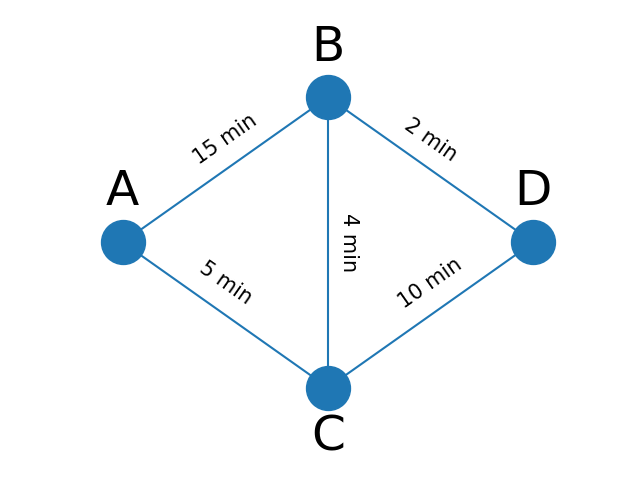
\includegraphics[width=\linewidth]{RoutePlanningProblem.png}
            \end{figure}
        \end{column}
    \end{columns}
\end{frame}

\begin{frame}{Example: Route Planning Problem}
    \textbf{First conceptualize the problem:}
    \begin{columns}
        \begin{column}{0.5\textwidth}
            \begin{figure}
                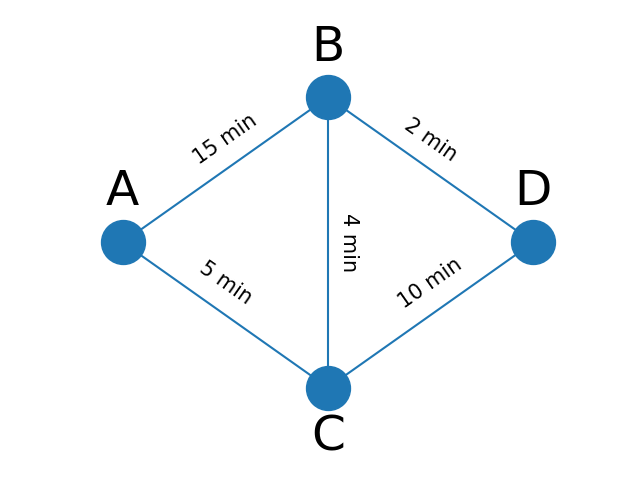
\includegraphics[width=\linewidth]{RoutePlanningProblem.png}
            \end{figure}
        \end{column}
        \begin{column}{0.5\textwidth}
            \begin{itemize}
                \item Objective: Minimize the time spent traveling
                \item Variables: 
                \begin{itemize}
                    \item Whether or not to travel down each stretch of road
                    \item Whether or not to visit each point
                \end{itemize}
                \item Parameters:
                \begin{itemize}
                    \item How long each stretch of road is
                    \item Which roads connect to which points
                \end{itemize}
                \item Constraints:
                \begin{itemize}
                    \item If I travel into a point, I must travel out of it.
                    \item I have to visit point A and point D
                \end{itemize}
            \end{itemize}
        \end{column}
    \end{columns}
\end{frame}

\begin{frame}[t]{Example: Route Planning Problem}
    \textbf{Then write the problem using mathematical modeling:}
    \begin{columns}[t]
        \begin{column}[t]{0.5\textwidth}
            \begin{enumerate}
                \item Define Sets:
                \begin{itemize}
                    \item $p \in \textbf{P} = \{A,B,C,D\}$: A set of all points
                    \item $p \in \textbf{P}^{NON-TERM} = \{B,C\}$: A set of all points other than the terminal (starting and ending) points
                    \item $p \in \textbf{P}^{TERM} = \{A,D\}$: A set of all the terminal points
                    \item $r \in \textbf{R} = \{AB,AC,BC,BD,CD\}$: A set of all roads
                    \item $r \in \textbf{R}_p$: A set of all roads that touch point $p$
                    
                    \begin{tabular}{|c|c|}
                        \hline
                        $p$ & $\textbf{R}_p$ \\
                        \hline \hline
                        $A$ & $\{AB,AC\}$\\
                        \hline
                        $B$ & $\{AB,BC,BD\}$\\
                        \hline
                        $C$ & $\{AC,BC,CD\}$\\
                        \hline
                        $D$ & $\{BD,CD\}$\\
                        \hline
                    \end{tabular}
                \end{itemize}
            \end{enumerate}
        \end{column}
        \begin{column}[t]{0.5\textwidth}
            \begin{enumerate}
                \setcounter{enumi}{1}
                \item Define Parameters:
                \begin{itemize}
                    \item $\delta_r$: The time it takes to travel road $r$
                    
                    \begin{tabular}{|c|c|}
                        \hline
                        $r$ & $\delta_r (minutes)$\\
                        \hline \hline
                        $AB$ & 15 \\
                        \hline
                        $AC$ & 5 \\
                        \hline
                        $BC$ & 4 \\
                        \hline
                        $BD$ & 2 \\
                        \hline
                        $CD$ & 10\\
                        \hline
                    \end{tabular}
                \end{itemize}

                \item Define Decision Variables:
                \begin{itemize}
                    \item $X_r \ \ \forall r \in \textbf{R}$: Whether or not to travel down road $r$ (\textbf{Binary Variable})
                    \item $Y_p \ \ \forall p \in \textbf{P}$: Whether or not to visit point $p$ (\textbf{Binary Variable})
                \end{itemize}
            \end{enumerate}
        \end{column}
    \end{columns}
\end{frame}

\begin{frame}[t]{Example: Route Planning Problem}
    \vspace{-0.2cm}
    \begin{columns}[t]
        \begin{column}[t]{0.5\textwidth}
            \begin{enumerate}
                \setcounter{enumi}{3}
                \item Define Constraints:
                \begin{itemize}
                    \item If I travel into a point, I must travel out of it 
                    $$\sum_{r \in \textbf{R}_p} X_r = 2 Y_p \ \ \ \forall p \in \textbf{P}^{NON-TERM}$$
                    $$\sum_{r \in \textbf{R}_p} X_r = Y_p \ \ \ \forall p \in \textbf{P}^{TERM}$$

                    \item I have to visit point A and point D
                    $$Y_p = 1 \ \ \ \forall p \in \textbf{P}^{TERM}$$
                \end{itemize}
                \item Define Objective:
                \begin{itemize}
                    \item Minimize the amount of time spent traveling
                    $$\min_{X_r,Y_p} \sum_{r \in \textbf{R}} \delta_r X_r$$
                \end{itemize}
            \end{enumerate}
        \end{column}
        \begin{column}[t]{0.5\textwidth}
            $$---\text{ FULL FORMULATION }---$$
            $$\min_{X_r,Y_p} \sum_{r \in \textbf{R}} \delta_r X_r$$
            $$s.t.\ \ \ \sum_{r \in \textbf{R}_p} X_r = 2 Y_p \ \ \ \forall p \in \textbf{P}^{NON-TERM}$$
            $$\sum_{r \in \textbf{R}_p} X_r = Y_p \ \ \ \forall p \in \textbf{P}^{TERM}$$
            $$Y_p = 1 \ \ \ \forall p \in \textbf{P}^{TERM}$$
            $$X_r, Y_p \in \{0,1\}$$

            \footnotetext{* Notice how the objective and all constraints are linear}
        \end{column}
    \end{columns}
\end{frame}


\begin{frame}[t]{Next Class}
    \begin{columns}[t]
        \begin{column}[t]{0.5\textwidth}
            \begin{itemize}
                \item Visit the course website:
            \end{itemize}
            \begin{figure}
                
\includegraphics[width=0.4\linewidth]{../CourseQRCode.png}
                \caption{QR Code to Course Website}
            \end{figure}
            \begin{itemize}
                \item These slides are posted in the Lecture 01 folder.
            \end{itemize}
        \end{column}
        \begin{column}[t]{0.5\textwidth}
            \begin{itemize}
                \item Python / Optimization coding crash course
                \item Go the the Lecture 02 folder on the course website
                \begin{itemize}
                    \item Follow the instructions on "slides.pdf" in the Lecture 02 folder.
                    \item The more you can do on your own before class the more time we'll have to answer questions and do example next class.
                \end{itemize}
                \item Please bring your laptops to class!
            \end{itemize}
        \end{column}
    \end{columns}
    %Bring computers
    %Have QR Code to Git Repo.
    %Tell them to follow slides to try to get python downloaded and ready to go before next class
    %Can I make a pre-made anaconda environment they can just download?

    %We'll do a crash course on Python and Pyomo
\end{frame}

\end{document}